\chapter{Αβεβαιότητες}\label{ch:uncert}
Έστω ότι μας δίνεται ένα φυσικό σύστημα και επιθυμούμε να σχεδιάσουμε ένα σύστημα
ελέγχου. Το πρώτο βήμα στο σχεδιασμό του συστήματος ελέγχου, είναι να περιγράψουμε
μαθηματικά το σύστημα βασιζόμενοι στους φυσικούς νόμους που διέπουν τη συμπεριφορά του.
Πολλές φορές, εμφανίζονται δυσκολίες που δυσχεραίνουν την ανάλυση του μοντέλου,
πχ μη γραμμικό σύστημα. Για το λόγο αυτό προσεγγίζουμε το σύστημα με γραμμικό και
σταθερών συντελεστών μοντέλο, που εκτιμούμε ότι προσεγγίζει ικανοποιητικά το πραγματικό
σύστημα. Τα συστήματα ελέγχου δηλαδή, σχεδιάζονται χρησιμοποιώντας μαθηματικά μοντέλα
τα οποία είναι μόνο προσεγγίσεις του πραγματικού συστήματος. Οι αποκλίσεις μεταξύ του
συστήματος και της μαθηματικής του περιγραφής μπορεί να οδηγήσουν σε μη
αποδεκτές επιδόσεις, ή ακόμα και σε αστάθεια του κλειστού συστήματος. Για να
περιγραφούν οι αποκλίσεις αυτές χρησιμοποιείται ο όρος \emph{αβεβαιότητα}.
Έτσι είναι απαραίτητο στοιχείο του σχεδιασμού να συμπεριληφθούν οι αβεβαιότητες του
συστήματος και η μοντελοποίηση ουσιαστικά, είναι ολοκληρωμένη μονάχα όταν έχουν ληφθεί
υπόψιν οι αβεβαιότητες αυτές.

Υπάρχουν διάφοροι λόγοι που μπορεί να εμφανιστούν αβεβαιότητες, κάποιοι από
αυτούς είναι:
\begin{enumerate}[label = (\enumgreek*)]
    \item Δεν γνωρίζουμε με ακρίβεια τις παραμέτρους του
        συστήματος που θέλουμε να ελέγξουμε.
    \item Η δυναμική του συστήματος μπορεί να μεταβάλλεται
        με το χρόνο, και η μεταβολή αυτή να μην έχει ληφθεί
        στη μοντελοποίηση.
    \item Τα περισσότερα συστήματα ελέγχου κατά το σχεδιασμό
        θεωρούνται γραμμικά και χρονικά αναλλοίωτα. Αυτό
        απλοποιεί μεν την ανάλυση και τον έλεγχο του συστήματος
        άλλα, στην πραγματικότητα όμως τα πραγματικά συστήματα
        είναι μη γραμμικά. Έτσι το γραμμικό σύστημα είναι απλά
        μία προσέγγιση του πραγματικού.
    \item Πολλές φορές εμφανίζονται συστήματα που είναι
        πολύπλοκη η περιγραφή της συμπεριφορά τους. Συνεπώς,
        δεν έχουμε άλλη επιλογή από το να χρησιμοποιήσουμε κάποια
        προσέγγιση αυτού.
    \item Εξωτερικές διαταραχές που δε δύναται να προβλεφθούν.
\end{enumerate}

Σύμφωνα με το βιβλίο~\cite{kosmidou2009robust}, οι αβεβαιότητες που εμφανίζονται
σε ένα σύστημα χωρίζονται σε δύο κατηγορίες, τις \emph{δομημένες αβεβαιότητες}
και τις \emph{μη δομημένες αβεβαιότητες}. Η μαθηματική περιγραφή των δομημένων
αβεβαιοτήτων είναι τέτοια ώστε γνωρίζουμε πως επηρεάζουν το σύστημα, και
συνήθως περιγράφονται στο πεδίο του χρόνου. Όσον αφορά τις μη δομημένες
αβεβαιότητες, καμία πληροφορία δεν είναι διαθέσιμη για το πως επιδρούν στο
σύστημα. Συνήθως περιγράφονται στο πεδίο της συχνότητας και η απόκλιση από
κάποια ονομαστική τιμή είναι φραγμένη από κάποιο άνω όριο. Ένα παράδειγμα δομημένης
αβεβαιότητας είναι κάποια παραμετρική μεταβολή στη δυναμική του μοντέλου, που
έχει ως αποτέλεσμα τη μεταβολή στα μηδενικά και στους πόλους της συνάρτησης μεταφοράς
του μοντέλου.  Παραδείγματα μη δομημένης αβεβαιότητας περιλαμβάνουν αβεβαιότητες
σχετικά με τη συχνότητα, όπως υψηλές συχνότητες που συνήθως αγνοούμε κατά τη
μοντελοποίηση ενός ταλαντωτή. Ένα ακόμα παράδειγμα μη δομημένης αβεβαιότητας είναι
η γραμμικοποίηση του μη γραμμικού συστήματος για να λάβουμε ένα γραμμικό απλούστερο μοντέλο.

Θα κάνουμε μία απλή αναφορά στις επικρατέστερες περιγραφές και
παραπέμπουμε στο βιβλίο~\cite{kosmidou2009robust} για περαιτέρω πληροφορίες.

Η περιγραφή στο πεδίο της συχνότητας, όπως αναφέραμε, είναι συνήθως μη
δομημένες και κάποιες περιγραφές είναι η περιγραφή με αθροιστική αβεβαιότητα,
η περιγραφή με πολλαπλασιαστική αβεβαιότητα στην είσοδο, η περιγραφή με
πολλαπλασιαστική αβεβαιότητα στην έξοδο, η περιγραφή με αντίστροφη πολλαπλασιαστική
αβεβαιότητα στην είσοδο, η περιγραφή με αντίστροφη πολλαπλασιαστική αβεβαιότητα
στην έξοδο. Επίσης, είναι δυνατή και μία δομημένη περιγραφή της αβεβαιότητας.

Η περιγραφή ενός αβέβαιου συστήματος στο χώρο καταστάσεων είναι
\begin{align*}
    \dot{x}(t) &= (A + \Delta A)x(t) + (B + \Delta B)u(t) \\
    y(t) &= (C + \Delta C)x(t) + (D + \Delta D)u(t),
\end{align*}
όπου οι πίνακες \( \Delta A, \Delta B, \Delta C \) και \( \Delta D \)
περιγράφουν τις αβεβαιότητες, που είναι μεταβολές των παραμέτρων του μοντέλου.
Θα θεωρήσουμε την περίπτωση όπου μόνο ο πίνακας κατάστασης είναι αβέβαιος.

Για την περίπτωση των μη δομημένων αβεβαιοτήτων έχουμε δύο περιγραφές. Τη
\emph{μη δομημένη παραμετρική αβεβαιότητα}. Ο πίνακας \( \Delta A \) περιέχει όλες τις
μεταβολές των παραμέτρων, χωρίς όμως να είναι γνωστή η δομή του, αλλά είναι
γνωστό ένα άνω φράγμα \( \|\Delta A\| \leq a \), όπου \( a \) κάποιο θετικό και
βαθμωτό μέγεθος. Την \emph{παραμετρική στοχαστική αβεβαιότητα}, όπου η αβεβαιότητα περιγράφεται
από κάποια στατιστικό μοντέλο.

Για την περίπτωση της δομημένης αβεβαιότητας, η
\emph{δομημένη παραμετρική αβεβαιότητα} είναι η συνηθέστερη. Οι επικρατέστερες
περιγραφές αυτής είναι οι ακόλουθες. Η \emph{γραμμική παραμετρική αβεβαιότητα},
όπου οι αβεβαιότητες είναι της μορφής
\[
    \Delta A = \sum_{i = 1}^k A_i p_i,
\]
όπου οι πίνακες \( A_i \) προσδιορίζουν τον τρόπο που επηρεάζει η αβεβαιότητα
στον πίνακα κατάστασης και \( p_i \) είναι μεταξύ ενός κάτω και ενός άνω ορίου.
Η \emph{πολυτοπική αβεβαιότητα}, όπου ο πίνακας κατάστασης ανήκει σε ένα
πολύτοπο που ορίζεται
\[
    A \in D_A = \{ A: A = \sum_{i = 1}^k A_i a_i, a_i \geq 0, \sum_{i = 1}^k a_i =
    1 \},
\]
όπου \( k \) είναι ο αριθμός των κορυφών του πολυέδρου \( D_A \).
Άλλες περιγραφές αβεβαιότητας είναι η \emph{αβεβαιότητα με φραγμένη νόρμα},
\emph{πραγματική θετική αβεβαιότητα} και η \emph{πραγματική φραγμένη
αβεβαιότητα}.

\section{Παράδειγμα αβέβαιου συστήματος}
Έστω το σύστημα
\begin{align*}
    \dot{x} &= Ax + Bu \\
    y &= Cx,
\end{align*}
όπου οι πίνακες \( A, B, C \) είναι
\[
    A =
    \begin{bmatrix}
        0 & 1 & 0 \\
        0 & 0 & 1 \\
        -1 & -3 & 2
    \end{bmatrix}, \quad
    B = \begin{bmatrix}0 \\ 0 \\ 1\end{bmatrix}, \quad
    C = \begin{bmatrix}1 & 1 & 1\end{bmatrix}.
\]
Το σύστημα είναι ασταθές, καθώς οι ιδιοτιμές του πίνακα κατάστασης
\( A \) είναι \( \lambda_{1,2,3} = -0.2757, 1.1378 + 1.5273i, 1.1378
- 1.5273i \) και έχουμε θετικό πραγματικό μέρος.

Για να σταθεροποιήσουμε το σύστημα θα κατασκευάσουμε ένα βέλτιστο τετραγωνικό
ελεγκτή απείρου χρόνου που ελαχιστοποιεί το δείκτη επίδοσης
\[
    J = \int_0^{\infty} \left( x^{T}Qx + u^{T}Ru \right) ,\ dt,
\]
με \( Q = I_3 \) και \( R = 1 \). Τρέχοντας την παρακάτω εντολή στο \tl{MATLAB}
με τους πίνακες όπως έχουν οριστεί παραπάνω
\eng{\begin{center}
        [K, S, e] = lqr(A, B, Q, R, N)
    \end{center}}
υπολογίζουμε το βέλτιστο κέρδος
\[
    K = \begin{bmatrix}0.4142 & 1.7127 & 4.9027\end{bmatrix}.
\]
Ο βέλτιστος νόμος ανάδρασης είναι \( u = -Kx \) που οδηγεί στο κλειστό σύστημα
με πίνακα κατάστασης
\[
    A_c = A - BK,
\]
που είναι ευσταθές, καθώς οι ιδιοτιμές του είναι
\( \lambda_{1,2,3} = -0.3758, -1.2634 + 1.4720i,
-1.2634 - 1.4720i \) και όλες έχουν αρνητικό πραγματικό μέρος.

Τώρα θεωρούμε ότι το σύστημα υπόκειται σε αβεβαιότητες που επηρεάζουν τον πίνακα
κατάστασης. Έστω ακόμα ότι η δομή της αβεβαιότητας είναι τέτοια που ο πίνακας
\( A \) γίνεται
\[
    A =
    \begin{bmatrix}
        0 & 1 & 0 \\
        0 & 0 & 1 \\
        -1 & -3 + r_1 & 2 + r_2
    \end{bmatrix},
\]
όπου \( r_1, r_2 \) εκφράζουν το εύρος της αβεβαιότητας. Σύμφωνα με τα όσα
είπαμε παραπάνω, βρισκόμαστε στην κατηγορία της γραμμικής παραμετρικής
αβεβαιότητας. Ο νέος πίνακας κατάστασης με την είσοδο των αβεβαιοτήτων μπορεί
να γραφτεί
\[
    A = A_0 + \Delta A_1 + \Delta A_2,
\]
όπου ο πίνακας \( A_0 \) είναι ο ονομαστικός πίνακας κατάστασης, δηλαδή ο
πίνακας του συστήματος χωρίς αβεβαιότητες και \( \Delta A_1, \Delta A_2 \) είναι
οι αβεβαιότητες. Έτσι αντικαθιστώντας τους πίνακες στην παραπάνω σχέση προκύπτει
\[
    A =
    \begin{bmatrix}
        0 & 1 & 0 \\
        0 & 0 & 1 \\
        -1 & -3 & 2
    \end{bmatrix} +
    \begin{bmatrix}
        0 & 0 & 0 \\
        0 & 0 & 0 \\
        0 & 1 & 0
    \end{bmatrix}r_1 +
    \begin{bmatrix}
        0 & 0 & 0 \\
        0 & 0 & 0 \\
        0 & 0 & 1
    \end{bmatrix}r_2.
\]

Μεταβάλλοντας τις αβεβαιότητες \( r_1, r_2 \) εντός του εύρους τιμών \( [-10,
10] \) μπορούμε να διαπιστώσουμε την επίδραση του κάθε ζεύγους \( (r_1, r_2) \)
στον πίνακα \( A \), όπως φαίνεται παραπάνω, και ως εκ τούτου στο σύστημα.
\begin{figure}[h]
    \centering
    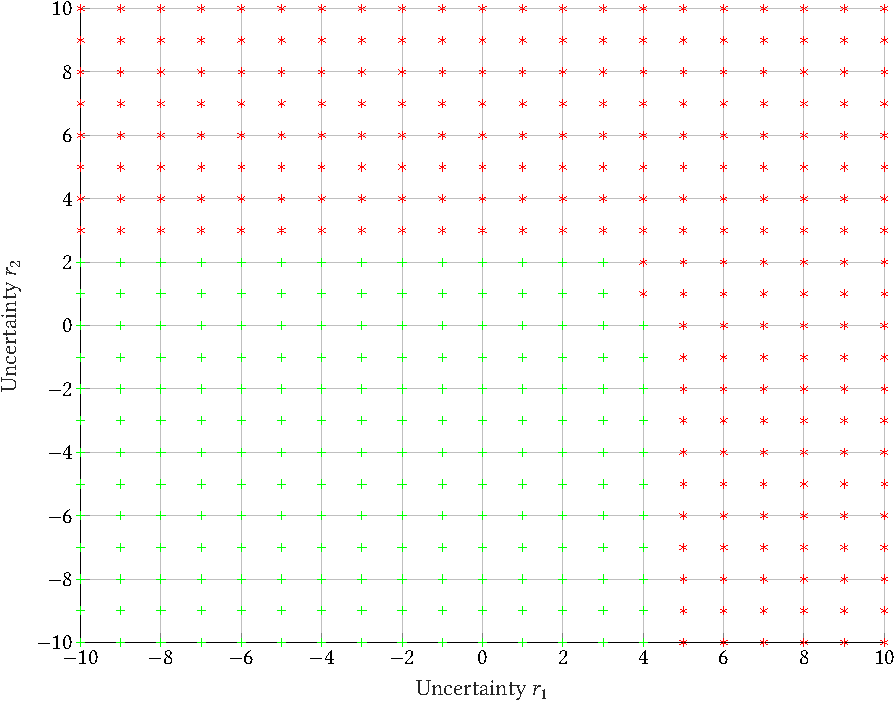
\includegraphics[width=0.9\textwidth]{figures/uncert_r.pdf}
    \captionG{Έλεγχος ευστάθειας συναρτήσει της μεταβολής των
    αβεβαιοτήτων \( r_1, r_2 \)}
    \label{fig:uncert_r}
\end{figure}
\begin{figure}[h]
    \centering
    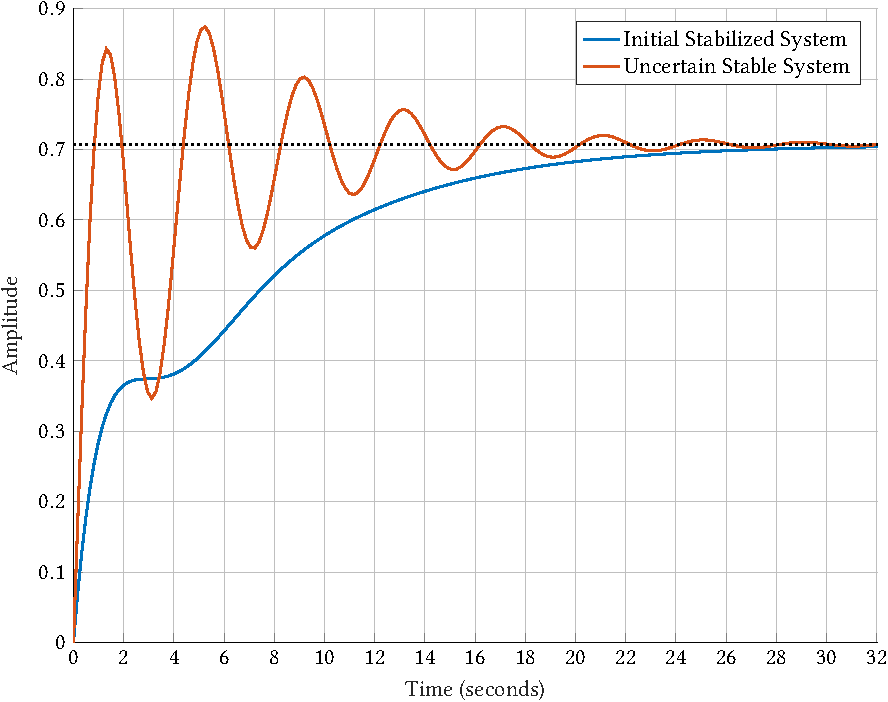
\includegraphics[width=0.9\textwidth]{figures/uncert_step.pdf}
    \captionG{Μοναδιαία βηματική απόκριση ονομαστικού και
    αβέβαιου συστήματος}
    \label{fig:uncert_step}
\end{figure}

Εφαρμόζοντας τη μεταβολή αυτή στο \tl{MATLAB}, προκύπτει το σχήμα~\ref{fig:uncert_r}.
Όπως παρατηρούμε τα ζεύγη τιμών κατά τα οποία μας δίνουν το πράσινο σταυρό,
είναι αυτά τα ζεύγη \( r_1, r_2 \) που δεν μετατρέπουν το ευσταθές σύστημα σε ασταθές.
Παρόλο αυτά με τη μεταβολή των αβεβαιοτήτων το σύστημα επηρεάζεται. Όσο αλλάζουν κατά
απόλυτη τιμή τα \( r_1, r_2 \) τόσο αποκλίνει το σύστημα από τους στόχους, είτε αυτοί είναι
γρήγορη σύγκλιση, μικρή υπερύψωση κτλ, μέχρι που καταλήγει να γίνει ασταθές.

Για να δούμε την επιρροή των αβεβαιοτήτων στο σύστημα παρουσιάζεται το
σχήμα~\ref{fig:uncert_step}. Το ζεύγος τιμών \( (r_1, r_2) = (2, 2) \) δε
μετατρέπει το αβέβαιο σύστημα σε ασταθές, όπως φαίνεται στο
σχήμα~\ref{fig:uncert_r}.
Παρόλο αυτά η επίδραση του στο σύστημα σε σχέση με το ονομαστικό είναι πολύ μεγάλη.
Οι ταλαντώσεις που δημιουργούνται είναι πολύ ισχυρές και ο χρόνος αποκατάστασης
μεγαλώνει αισθητά. Καταλαβαίνουμε δηλαδή ότι βρισκόμαστε κοντά σε ασταθή
κατάσταση.

Παρακάτω παρατίθεται ο κώδικας στο \tl{MATLAB} που χρησιμοποιήθηκε για το
παράδειγμα.
\eng{\lstinputlisting[language=Matlab]{src/uncert.m}}
